%!TEX root=../../main.tex
\begin{chapterpage}{One--sample hypothesis testing}
  \chaptertitle{One--sample hypothesis testing}
  \label{ch:OneSampleHT}
 % \chaptersection{variabilityInEstimates}
 % \chaptersection{confidenceIntervals}

  \chaptersection{hypothesisTesting}
  \chaptersection{HTofMean}
  \chaptersection{HTofProportion}
  \chaptersection{UnderstandingHT}
  \chaptersection{ch5Summary}
 \chaptersection{ch5Exercises}
\end{chapterpage}
\renewcommand{\chapterfolder}{ch_05a_inference_foundations_oi_biostat}

\chapterintro{
  This chapter introduces  a method for testing scientific hypotheses about $\mu$. The concepts used in this chapter will appear throughout the rest of the book, for other settings of hypotheses.

  
In this chapter hypothesis testing  will be applied to three cases related to veterinary : 
\begin{enumerate}
\item Analyzing the effect of vegetarian diet in pigs and compare the weight of a vegetarian pigs and the weight of a pigs which eat typical animal feed.
\item Comparing heart rate of dogs living close to a heavy traffic road with the usual heart rate. 
\item Checking whether there exists any difference between the prevalence of  a parasitic disease in a country with another country whose data are corroborated by several studies. 
\end{enumerate}
}
%%%% CAMBIO: SE HAN BORRADO LAS SECCIONES CORRESPONDIENTE A OTROS CAPITULOS

%__________
\section[Hypothesis testing]{Hypothesis testing} %\sectionvideohref{youtube-NVbPE1_Cbx8&list=PLkIselvEzpM7Pjo94m1e7J5jkIZkbQAl4}}
\label{hypothesisTesting}

\index{hypothesis testing|(}

Important decisions in science, such as whether a new treatment for a disease should be approved for the market, are primarily data-driven. For example, does a clinical study of a new cholesterol-lowering drug provide robust evidence of a beneficial effect in patients at risk for heart disease? A confidence interval can be calculated from the study data to provide a plausible range of values for a population parameter, such as the population average decrease in cholesterol levels. A drug is considered to have a beneficial effect on a population of patients if the population average effect is large enough to be clinically important. It is also necessary to evaluate the strength of the evidence that a drug is effective; in other words, is the observed effect larger than would be expected from chance variation alone?

Hypothesis testing is a method for calculating the probability of making a specific observation under a working hypothesis, called the null hypothesis. By assuming that the data come from a distribution specified by the null hypothesis, it is possible to calculate the likelihood of observing a value as extreme as the one represented by the sample. If the chances of such an extreme observation are small, there is enough evidence to reject the null hypothesis in favor of an alternative hypothesis. 

\begin{onebox}{Null and alternative hypotheses}
  {The \term{null hypothesis ($H_0$)} often represents either a skeptical perspective or a claim to be tested. The \term{alternative hypothesis ($H_A$)} is an alternative claim and is often represented by a range of possible parameter values.}
\end{onebox}

Generally, an investigator suspects that the null hypothesis is not true and performs a hypothesis test in order to evaluate the strength of the evidence against the null hypothesis. The logic behind rejecting or failing to reject the null hypothesis is similar to the principle of presumption of innocence in many legal systems. In the United States, a defendant is assumed innocent until proven guilty; a verdict of guilty is only returned if it has been established beyond a reasonable doubt that the defendant is not innocent. In the formal approach to hypothesis testing, the null hypothesis ($H_0$) is not rejected unless the evidence contradicting it is so strong that the only reasonable conclusion is to reject $H_0$ in favor of $H_A$. 

We could use a reasoning based on confidence intervals as it is shown in the next example. 
\index{data!Great Danes|(}

 \begin{examplewrap}
 \begin{nexample}{The heart rate   is known to
 have a mean value of   90 for  Great Dane dogs in normal conditions.\footnote{Disclaim: These data are not real. They are generated in order to provide an example, but has nothing to do with the true heart rate of a dog.} We try to verify if there is any difference between the heart rate for dogs living in a noisy neighbourhood and another dog living in a quieter neighbourhood.  With this purpose, we have randomly selected  10 Great Danes living close to heavy traffic road the  
 number of beats per minutes are the following:
 \begin{center}
   113, 95, 97, 107, 85, 100, 100, 115, 98, 112 
 \end{center}} 
\label{ex:GreatDanesCI}

 We need to assume that the heart rate is normally distributed in order to be able to calculate a confidence interval.  
 We set up the hypothesis where $\mu$ is the aveage heart rate of dogs living close to heavy traffic area: 
 \begin{itemize}
 \item[$H_0$:] The heart rate of Great Danes living close to heavy traffic area is the same that the average heart rate of the general population, $\mu=90$ 
 \item[$H_A$:] The heart rate of Great Danes living close to heavy traffic area isdifferent from the average heart rate of the general population, $\mu=90$ 
 \end{itemize}

   The sample size is 10, the sample mean is 102.2 and the sample variance is 82.0667. Hence, the estimation of the standard error is $SE=\sqrt{89.0667/10}=2.9884$. We can construct a 95\% confidence interval by means of the t distribution since population variance is unknown.    
 $$\bar{x}\pm t_{9,.975}SE=102.2\pm2.262 \cdot 2.9884 \quad \to \quad (95.4402,108.9598)$$
 The value 90 does not belong to the interval and if the null hipothesis were true and the average heart rate were 90, this event would happen less than 5\% of the times. Therefore, there exists evidence that the average heart rate is different from 90. 

 \index{data!Great Danes|)} 
 \end{nexample}
 \end{examplewrap}
In health and biological science is preferred to follow  the steps in formal hypothesis testing presented in the next section, which is applied when data are analyzed to support a decision or make a scientific claim.


\subsection{The Formal Approach to Hypothesis Testing}
\label{formalHypothesisTesting}

In this section, hypothesis testing will be used to address the question of whether Americans generally wish to be heavier or lighter than their current weight. In the \data{cdc} data, the two variables \var{weight} and \var{wtdesire} are, respectively, the recorded actual and desired weights for each respondent, measured in pounds. 

Suppose that $\mu$ is the population average of the difference \texttt{weight} $-$ \texttt{wtdesire}. Using the observations from \data{cdc.samp}, assess the strength of the claim that, on average, there is no systematic preference to be heavier or lighter.

There are two techniques to apply hypothesis testing, one of them is based on calculating a p-value and the other one an acceptance interval. The technique of the p-value is difficul to apply when using tables except for a big sample, but statistical software, such as R-Commander, display this value and the conclusion must be drawn from it.  


%\textD{\newpage}


\subsubsection{Step 1: Formulating null and alternative hypotheses}

The claim to be tested is that the population average of the difference between actual and desired weight for US adults is equal to 0. 
\[H_0: \mu = 0.\]

In the absence of prior evidence that people typically wish to be lighter (or heavier), it is reasonable to begin with an alternative hypothesis that allows for differences in either direction.
\[H_A: \mu \neq 0.\]

The alternative hypothesis $H_A: \mu \neq 0$ is called a \term{two-sided alternative}. A one-sided alternative could be used if, for example, an investigator felt there was prior evidence that people typically wish to weigh less than they currently do: $H_A: \mu > 0$. 

More generally, when testing a hypothesis about a population mean $\mu$, the null and alternative hypotheses are written as follows
\begin{itemize}
\setlength{\itemsep}{0mm}
  \item For a two-sided alternative:
    \[H_0: \mu = \mu_0, \ H_A: \mu \neq \mu_0.\]    
  \item For a one-sided alternative:
    \[H_0: \mu = \mu_0, \ H_A: \mu < \mu_0
      \qquad\text{or}\qquad
      H_0: \mu = \mu_0, \  H_A: \mu > \mu_0.\]
\end{itemize}
The symbol $\mu$ denotes a population mean, while $\mu_0$ refers to the numeric value specified by the null hypothesis; in this example, $\mu_0 = 0$ (no difference between deired cand real weight). Note that null and alternative hypotheses are statements about the underlying population, not the observed values from a sample.
% CAMBIO Se ha aclarado cual es la `response variable' 
The \term{response variable} is the used to calculate the mean or any other parameter, such as proportion.

\subsubsection{Step 2: Specifying a significance level, $\alpha$}

It is important to specify how rare or unlikely an event must be in order to represent sufficient evidence against the null hypothesis. This should be done during the design phase of a study, to prevent any bias that could result from defining 'rare' only after analyzing the results. 

When testing a statistical hypothesis, an investigator specifies a \term{significance level}, $\alpha$, that defines a 'rare' event. Typically, $\alpha$ is chosen to be $0.05$, though it may be larger or smaller, depending on context; this is discussed in more detail in Section~\ref{significanceLevel}. An $\alpha$ level of $0.05$ implies that an event occurring with probability lower than 5\% will be considered sufficient evidence against $H_0$.


\subsubsection{Step 3: Calculating the test statistic}
A \emph{test statistic} is a special summary statistic that is particularly useful for evaluating a hypothesis test or identifying the p-value. In general, it has the form 
$$  \frac{\text{point estimate}- \text{null value}}{SE_{\text{point estimate}}}$$


Therefore, calculating the test statistic $t$ is analogous to standardizing observations with Z-scores. For a hypothesis testing of the mean, the mean  test statistic quantifies the number of standard deviations between the sample mean $\overline{x}$ and the population mean $\mu$:
\begin{align*}
t=\frac{\overline{x}-\mu_0}{s/\sqrt{n}},
\end{align*}
where $s$ is the sample standard deviation and $n$ is the number of observations in the sample.  If $x =$ \texttt{weight} $-$ \texttt{wtdesire}, then for the 60 recorded differences in \data{cdc.samp}, $\overline{x} = 18.2$ and $s = 33.46$.  In this sample, respondents weigh on average about 18\,lbs more than they wish. The test statistic is 
\[t = \frac{18.2 - 0}{33.46/\sqrt{60}} = 4.22.\]
The observed sample mean is 4.22 standard deviations to the right of $\mu_0 = 0$.


%\textD{\newpage}


\subsubsection{Step 4 (for large sample): Calculating the $\pmb{\MakeLowercase{p}}$-value}

The \termsub{$\pmb{\MakeLowercase{p}}$-value}{p-value} is the probability of observing a sample mean as or more extreme than the observed value, under the assumption that the null hypothesis is true. In samples of size 40 or more, the $t$-statistic will have a standard normal distribution unless the data are strongly skewed or extreme outliers are present. Recall that a standard normal distribution has mean 0 and standard deviation 1.

For two-sided tests, with $H_A: \mu \neq \mu_0$, the $p$-value is the sum of the area of the two tails defined by the $t$-statistic: $2 P(Z \geq |t|) = P(Z \leq -|t|) + P(Z \geq |t|)$ (Figure~\ref{pValueTwoSided}).

\begin{figure}[h]
	\centering
	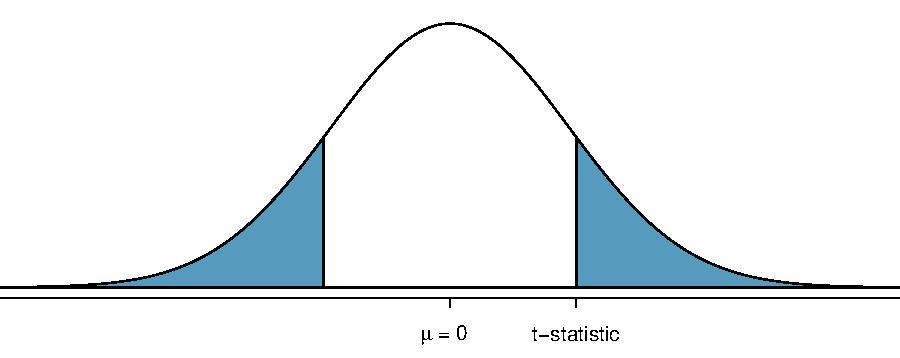
\includegraphics[width=0.9\textwidth]{ch_05a_inference_foundations_oi_biostat/figures/pValueTwoSided/pValueTwoSided}
	\caption{A two-sided $p$-value for $H_A: \mu \neq \mu_0$ on a standard normal distribution. The shaded regions represent observations as or more extreme than $\overline{x}$ in either direction.}
	\label{pValueTwoSided}
\end{figure}

For one-sided tests with $H_A: \mu > \mu_0$, the $p$-value is given by $P(Z \geq t)$, as shown in Figure~\ref{pValueOneSided}. If $H_A: \mu < \mu_0$, the $p$-value is the area to the left of the $t$-statistic, $P(Z \leq t)$.

\begin{figure}[h]
	\centering
	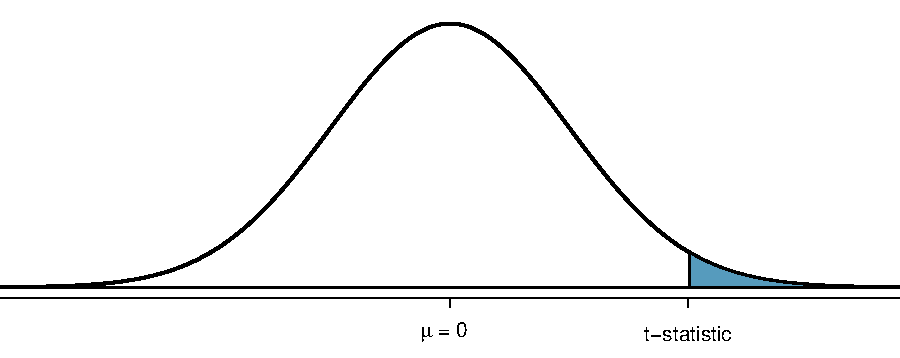
\includegraphics[width=0.9\textwidth]{ch_05a_inference_foundations_oi_biostat/figures/pValueOneSided/pValueOneSided}
	\caption{A one-sided $p$-value for $H_A: \mu > \mu_0$ on a standard normal distribution is represented by the shaded area to the right of the $t$-statistic. This area equals the probability of making an observation as or more extreme than $\overline{x}$, if the null hypothesis is true.}
	\label{pValueOneSided}
\end{figure}


The $p$-value can either be calculated from software or from the normal probability tables. For the weight-difference example, the $p$-value is vanishingly small: $p = P(Z \leq - 4.22) + P(Z > 4.22)< 0.001$.


%\textD{\newpage}

\subsubsection{Step 4 (for any sample): Calculate acceptance interval}

Instead of calculating p-value, which is always possible to calculate with an adequate software, set an interval containing the values for which the null hypothesis is failed to reject. The decision is make depending on the value being inside or outside the interval. This interval is calculated with percentiles of the distribution of the test statistic, pay attention that the distribution of the test statistic is not the same as the response variable. 

The critical value(s) define the
    \emph{rejection area} is the range the values of the test
    statistic for which is said the test result is statistically
    significant and the test hypothesis rejected.

  The \emph{acceptance region} is the range of values of a test
  statistics for which there is not enough statistical evidence to
  reject the null hypotheses. So, the null hypothesis is failed to reject  For the two-sided tests, if the sample is small, the acceptance interval is given by percentiles of the t distribution $(-t_{n-1,1-\alpha/2}, t_{n-1,1-\alpha/2})$ and if the sample is large enough, the acceptance interval is given by percentile of the normal distribution, $(-z_{1-\alpha/2}, z_{1-\alpha/2})$. 


\subsubsection{Step 5: Drawing a conclusion}

To reach a conclusion about the null hypothesis, directly compare $p$ and $\alpha$. Note that for a conclusion to be informative, it must be presented in the context of the original question; it is not useful to only state whether or not $H_0$ is rejected.

If $p > \alpha$, the observed sample mean is not extreme enough to warrant rejecting $H_0$; more formally stated, there is insufficient evidence to reject $H_0$. A high $p$-value suggests that the difference between the observed sample mean and $\mu_0$ can reasonably be attributed to random chance.

If $p \leq \alpha$, there is sufficient evidence to reject $H_0$ and accept $H_A$. In the \data{cdc.samp} weight-difference data, the $p$-value is very small, with the $t$-statistic lying to the right of the population mean. The chance of drawing a sample with mean as large or larger than 18.2 if the distribution were centered at 0 is less than 0.001. Thus, the data support the conclusion that on average, the difference between actual and desired weight is  not 0 and is positive; people generally seem to feel they are overweight.

% CAMBIO: anyadido que hacer con acceptance interval
If the acceptance interval is calculated in step~4, null hypothesis is rejected if test statistic is outside the interval. Otherwise, the null hypothesis is failed to reject.   

\begin{exercisewrap}
\begin{nexercise}
Suppose that the mean weight difference in the sampled group of 60 adults had been 7 pounds instead of 18.2 pounds, but with the same standard deviation of 33.46 pounds. Would there still be enough evidence at the $\alpha = 0.05$ level to reject $H_0: \mu = 0$ in favor of $H_A: \mu \neq 0$?\footnotemark{}
\end{nexercise}
\end{exercisewrap}
\footnotetext{Re-calculate the $t$-statistic: $(7 - 0)/(33.46/\sqrt{60}) = 1.62$. The $p$-value $ P(Z \leq -1.62) + P(Z \geq 1.62) = 0.105$. Since $p$ > $\alpha$, there is insufficient evidence to reject $H_0$. In this case, a sample average difference of 7 is not large enough to discount the possibility that the observed difference is due to sampling variation, and that the observations are from a distribution centered at 0.}


%\textD{\newpage}

\section{Hypothesis testing of the mean}
\label{HTofMean}

If the null hypothesis refers to the mean of a response varible to a \term{reference value} $\mu_0$, the test statistic to use is $t= \frac{\overline{x}-\mu_0}{s/\sqrt{n}}$, called $t$-test statistic.
We have to pay attention to the response variable and the sample size to determine its distribution. If the sample size is large enough, mamely $n>30$ and not very skewed, the $t$-test statistic is very close to follow a standard normal distribution. If the response variable is normally distributed, then  the $t$-test statistic follows a Student's t distribution with $n-1$ degrees of freedom. Consequently, if the sample is small and the response variable is clearly not normally distributed, we cannot apply neither normal distribution nor t-distribution. However, if it is a large sample and the response variable is normally distributed, using normal distribution or t-distribution are almost equivalent.

\subsection{Two examples with large samples \vspace{-3mm}}



\begin{examplewrap}
\begin{nexample}{In 2015, the National Sleep Foundation published new guidelines for the amount of sleep recommended for adults: 7-9 hours of sleep per night.\footnotemark{} The NHANES survey includes a question asking respondents about how many hours per night they sleep; the responses are available in \data{nhanes.samp}. In the sample of 134 adults used in the BMI example, the average reported hours of sleep is 6.90, with standard deviation 1.39. Is there evidence that American adults sleep less than 7 hours per night?}

Let $\mu$ be the population average of hours of sleep per night for US adults. Conduct a one-sided test, since the question asks whether the average amount of sleep per night might be less than 7 hours. 

\textit{Formulate the null and alternative hypotheses}. $H_0: \mu = 7$ hours vs. $H_A: \mu < 7$ hours.

\textit{Specify the significance level, $\alpha$}.  Let $\alpha = 0.05$, since the question does not reference a different value. 

\textit{Calculate the test statistic}. The $t$-statistic has value
\[t = \frac{\overline{x}-\mu_0}{s/\sqrt{n}} = \frac{6.90 - 7.00} {1.33/\sqrt{134}} = -0.864.\]

\textit{Calculate the $p$-value}.

For this one-sided alternative $H_A: \mu < 7$, the $p$-value is
\[P(Z \leq t) = P(Z < -0.864) = 0.19.\]

Since the alternative states that $\mu_0$ is less than 7, the $p$-value is represented by the area to the left of $t = -0.864$, as shown in Figure~\ref{pValueSleep}.

\textit{Draw a conclusion}.  The $p$-value is larger than the specified significance level $\alpha$. The null hypothesis is not rejected since the data do not represent sufficient evidence to support the claim that American adults sleep less than 7 hours per night.
\end{nexample}
\end{examplewrap}
\footnotetext{Sleep Health: Journal of the National Sleep Foundation, Vol. 1, Issue 1, pp. 40 - 43}

%\textD{\newpage}

\begin{figure}[h]
	\centering
	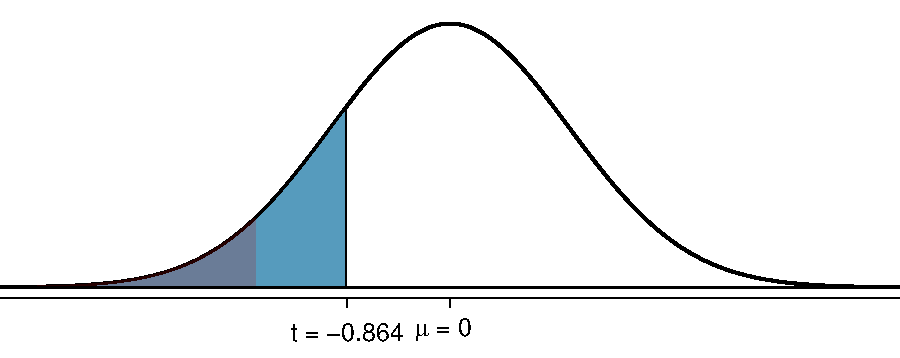
\includegraphics[width=0.85\textwidth]{ch_05a_inference_foundations_oi_biostat/figures/pValueSleep/pValueSleep}
	\caption{The large blue shaded region represents the $p$-value, the area to the left of $t = -0.864$. The smaller grey shaded region represents the rejection region of area 0.05 in the left tail.}
	\label{pValueSleep}
\end{figure}

\begin{exercisewrap}
\begin{nexercise}
From these data, is there sufficient evidence at the $\alpha = 0.10$ significance level to support the claim that American adults sleep more than 7 hours per night?\footnotemark{}
\end{nexercise}
\end{exercisewrap}
\footnotetext{The $t$-statistic does not change from 1.65. Re-calculate the $p$-value since the alternative hypothesis is now $H_A: \mu > 7$: $P(Z \geq -0.864) = 0.81$. Since $p$ > $\alpha$, there is insufficient evidence to reject $H_0$ at $\alpha = 0.10$. A common error when conducting one-sided tests is to assume that the $p$-value will always be the area in the smaller of the two tails to the right or left of the observed value. It is important to remember that the area corresponding to the $p$-value is in the direction specified by the alternative hypothesis.\\
	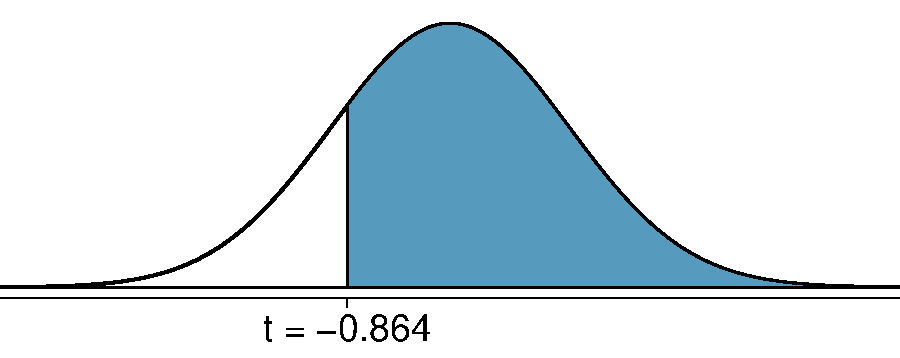
\includegraphics[width=0.45\textwidth]{ch_05a_inference_foundations_oi_biostat/figures/pValueSleep/pValueSleepEx}}


  
\begin{examplewrap}
\begin{nexample}{It is known that the general population of pigs bred on farms have a
average weight of 57 kg after 6 month. What happen with pigs which are
feed with a vegetarian diet. He have collected 100 pigs 6 months-old fed
with a vegetarian diet and the average weight was 55.9 kg and the
standard deviation was 5\,Kg. Is there any significant difference? }
We can apply the normal model since we have the conditions of independent\footnote{A  remark of caution: Independence could be compromised if our sample were extracted from just a few farms instead of all the farms which are providing vegetarian diet. Since they are sharing conditions like temperatute, room, etc, two pigs from the same farm would not be completely  independent. } and the sample size being larger than 30. We assume that the distribution is unskewed, in case of being provided the  data set a histogram should be generated to check that they are not strongly skewed. 

The null hypothesis would be the skeptical point of view that the type of diet has nothing to do with the weight and the alternative would be that pigs fed with vegetarian diet have a lower weight.
\begin{itemize}
\item[$H_0$] The average weight of pigs fed with vegetarian diet is the same that pigs fed with the usual animal feed, $\mu=57$.
\item[$H_1$] The average  weight of pigs fed with vegetarian diet is smaller than average weight for pigs fed with the usual animal feed, $\mu<57$.  
\end{itemize}
The $t$-statistics test will be $t=\frac{\bar{x}-\mu_0}{s/\sqrt{n}}=\frac{55.9-57}{5/\sqrt{100}}=-2.2$. The p--value is the probability of getting a value lower than this value if the null hypothesis is true. Hence, the p--value is the probability of a standard normal variable will be lower than $-2.2$, so is the lower tail area of the normal distribution. 
$$P(Z<-2.2)=1-P(Z<2.2)=1-0.9861=0.0139$$ 
This p-value is lower that $\alpha=0.05$. We can consider that there exists a significant difference and that there is evidence that the average weight of pigs fed with vegetarian diet is smaller than the averaged weight of pigs eating the usual animal feed.
\end{nexample}
\end{examplewrap}

      \subsection{Examples with small samples}
      
\begin{examplewrap}
\begin{nexample}{While fish and other types of seafood are important for a healthy diet, nearly all fish and shellfish contain traces of mercury. Dietary exposure to mercury can be particularly dangerous for young children and unborn babies. Regulatory organizations such as the US Food and Drug Administration (FDA) provide guidelines as to which types of fish have particularly high levels of mercury and should be completely avoided by pregnant women and young children; additionally, certain species known to have low mercury levels are recommended for consumption. While there is no international standard that defines excessive mercury levels in saltwater fish species, general consensus is that fish with levels above 0.50 parts per million (ppm) should not be consumed. A study conducted to assess mercury levels for saltwater fish caught off the coast of New Jersey found that a sample of 23 bluefin tuna had mean mercury level of 0.52 ppm, with standard deviation 0.16 ppm.\footnote{J. Burger, M. Gochfeld, Science of the Total Environment 409 (2011) 1418–1429} Based on these data, should the FDA add bluefin tuna from New Jersey to the list of species recommended for consumption, or should a warning be issued about their mercury levels?}\label{hypTestTuna}%
Let $\mu$ be the population average mercury content for bluefin tuna caught off the coast of New Jersey. Conduct a two-sided test of the hypothesis $\mu = 0.50$ ppm in order to assess the evidence for either definitive safety or potential danger.

\textit{Formulate the null and alternative hypotheses}. $H_0: \mu = 0.50$ ppm vs. $H_A: \mu \neq 0.50$ ppm

\textit{Specify the significance level, $\alpha$}.  A significance level of $\alpha = 0.05$ seems reasonable. 

\textit{Calculate the test statistic}. The  $t$-statistic has value
\begin{align*}
t &= \frac{\overline{x}-\mu_0}{s/\sqrt{n}} = \frac{0.52 - 0.50} {0.16/\sqrt{23}} = 0.599.
\end{align*}

\textit{Calculate the acceptance interval} \footnote{The p-value could be calculated using statistical software. The value is $2\times P(t_{22}>0.599)=2\times 0.2776=0.5552$}. For a small sample, a response variable normally distributed and a two-sided alternative $H_A: \mu \neq 0.50$, the response variable is following the Student's t-distribution with $df=n-1=22$ degrees of freedom, on the table $t_{df,1-\alpha/2}=t_{22,0.975}=2.074$, So, the acceptance interval is  $(-2.074,2.074)$.

% \[P(Z \leq -|t|) + P(Z \geq |t|) = 2 \times P(Z \geq 0.599) = 0.549.\]

\textit{Draw a conclusion}. \footnote{The $p$-value is larger than the specified significance level $\alpha$, as shown in Figure~\ref{pValueTuna}. The data do not show that the mercury content of bluefin tuna caught off the coast of New Jersey differs significantly from 0.50 ppm. Since $p > \alpha$, there is insufficient evidence to reject the null hypothesis} The $t$-test statistic is not included in the acceptance interval, therefore there is not enough evidence to reject  that the mean mercury level for the New Jersey coastal population of bluefin tuna is 0.50 ppm. 

Note that "failure to reject" is not equivalent to "accepting" the null hypothesis. Recall the earlier analogy related to the principle of "innocent until proven guilty". If there is not enough evidence to prove that the defendant is guilty, the official decision must be "not guilty", since the defendant may not necessarily be innocent. Similarly, while there is not enough evidence to suggest that $\mu$ is not equal to 0.5 ppm, it would be incorrect to claim that the evidence states that $\mu$ \textit{is} 0.5 ppm.

From these data, there is not statistically significant evidence to either recommend these fish as clearly safe for consumption or to warn consumers against eating them. Based on these data, the Food and Drug Administration might decide to monitor this species more closely and conduct further studies. 
\end{nexample}
\end{examplewrap}
%\addtocounter{footnote}{-1}%
%\footnotetext{J. Burger, M. Gochfeld, Science of the Total Environment 409 (2011) 1418–1429}%
%\addtocounter{footnote}{1}%
%\footnotetext{The grey shaded regions are bounded by -1.96 and 1.96, since the area within 1.96 standard deviations of the mean captures 95\% of the distribution.}

\begin{figure}[h]
	\centering
	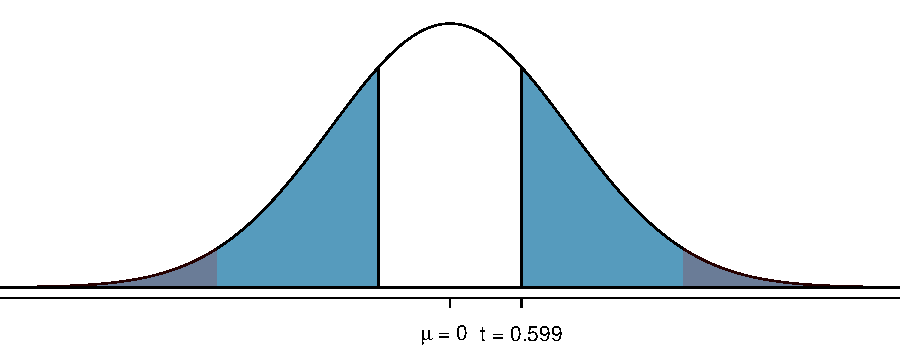
\includegraphics[width=0.9\textwidth]{ch_05a_inference_foundations_oi_biostat/figures/pValueTuna/pValueTuna}
	\caption{The large blue shaded regions represent the $p$-value, the area to the right of $t = 0.599$ and to the left of $-t = -0.599$. The smaller grey shaded regions represents the \term{rejection region} as defined by $\alpha$; in this case, an area of 0.025 in each tail. The $t$-statistic calculated from $\overline{x}$ would have to lie within either of the extreme tail areas to constitute sufficient evidence against the null hypothesis. The grey shaded regions are bounded by -2.074 and 2.074,  capturing 95\% of the distribution of the test statistic.}
	\label{pValueTuna}
\end{figure}  

\index{data!Great Danes|(}
\begin{examplewrap}
\begin{nexample} {Use the data in exercise~\ref{ex:GreatDanesCI} to check whether the heart rate of Great Danes living close to a heavy traffic road is different from the average  heart rate. With a significance level of $\alpha=0.05$}
We assume that the distribution of the heart rate is normally distributed\footnote{In general, this procedure for hypothesis testing works if the distribution of the variable is symmetric. }
 We standarize with the same way than $z$, but we use the $t$ statistic in order to indicate that this test statistic is using Student's t distribution.  
$$t=\frac{\bar{x}-\mbox{null value}}{SE}= \frac{102.2-90}{9.43/\sqrt{10}}=\frac{102.2-90}{2.98}=4.09$$
The acceptance interval is $(-t_{9,.975},t_{9,.975})=(-2.262,2.262)$. The value of the test statistic does not belong to the interval. Therefore, null hypothesis is rejected and we have enough statistical evidence that there exists a difference between the average value of the heart rate of Great Danes living near heavy traffic roads and the general average heart rate for these dogs.
\end{nexample}
\end{examplewrap}
\index{data!Great Danes|)}

      
  %% CAMBIO: Seccion de la relacion entre intervalo de confianza y HT eliminada. 

\section{Hypothesis testing of proportions}
\label{HTofProportion}

\index{hypothesis testing!single proportion}

Just as with inference for population means, confidence intervals for population proportions can be used when deciding whether to reject a null hypothesis. It is useful in most settings, however, to calculate the $p$-value for a test as a measure of the strength of the evidence contradicting the null hypothesis.

When using the normal approximation for the distribution of $\hat{p}$ to conduct a hypothesis test, one should always verify that $\hat{p}$ is nearly normal under $H_0$ by checking the independence and success-failure conditions. Since a hypothesis test is based on the distribution of the test statistic under the null hypothesis, the success-failure condition is checked using the null proportion $p_0$, not the estimate $\hat{p}$. 

According to the normal approximation to the binomial distribution, the number of successes in $n$ trials is normally distributed with mean $np_0$ and standard deviation $\sqrt{np_0(1-p_0)}$. This approximation is valid when $np_0$ and $n(1-p_0)$ are both at least 10.%\footnote{The normal approximation to the binomial distribution was discussed in Section~\ref{binomialModel} of Chapter~\ref{modeling}.} 

%\textD{\newpage}

Under the null hypothesis, the sample proportion $\hat{p} = X/n$ is approximately distributed as 
\[N \left(p_0, \sqrt{\frac{p_0(1-p_0)}{n}} \right).\]
The test statistic $z$ for the null hypothesis $H_0: p = p_0$ based on a sample of size $n$ is 
\begin{align*}
  z &= \dfrac{\text{point estimate - null value}}{SE} =\dfrac{\hat{p} - p_0}{\sqrt{\frac{(p_0)(1-p_0)}{n}}}. 
\end{align*}

\begin{examplewrap}
\begin{nexample}{Suppose that out of a cohort of 120 patients with stage 1 lung cancer at the Dana-Farber Cancer Institute (DFCI) treated with a new surgical approach, 80 of the patients survive at least 5 years, and suppose that National Cancer Institute statistics indicate that the 5-year survival probability for stage 1 lung cancer patients nationally is 0.60. Do the data collected from 120 patients support the claim that the DFCI population treated with this new form of surgery has a different 5-year survival probability than the national population? Let $\alpha = 0.10$, since this is an early study of the new surgery.}

Test the hypothesis $H_0: p = 0.60$ versus the alternative, $H_A:  p \neq 0.60$, using $\alpha = 0.10$. If we assume that the outcome of one patient at DFCI does not influence the outcome of other patients, the independence condition is met, and the success-failure condition is satisfied since $(120)(0.60) = 80 > 5$ and $(120)(1-0.60) = 40 > 5.$ The test statistic is the $z$-score of the point estimate: 
\[z = \dfrac{\text{point estimate - null value}}{SE} = \dfrac{0.67 - 0.60}{\sqrt{\frac{(0.60)(1-0.60)}{120}}} = 1.57. \]
The $p$-value\footnote{The technique of the acceptance interval could be used by means of percentiles of the normal distribution  $(-z_{1-\alpha/2} , z_{1-\alpha/2} )$. Since $z_{0.95}=1.645$, the acceptance interval is $(-1.645,1.645)$}is the probability that a standard normal variable is larger than 1.57 or smaller than -1.57, $P(|Z| > 1.57) = 0.12$ ; since the $p$-value is greater than 0.10, there is insufficient evidence to reject $H_0$ in favor of $H_A$. There is not convincing evidence that the survival probability at DFCI differs from the national survival probability.  Had a more traditional 0.05 significance level been used, the data would be even less convincing. 
\end{nexample}
\end{examplewrap}

\begin{examplewrap}
\begin{nexample}{Using the data from the study in advanced melanoma, use the normal approximation to the sampling distribution of $\hat{p}$ to test the null hypothesis that the response probability to the novel combined therapy is 30\% against a one-sided alternative that the response proportion is greater than 30\%. Let $\alpha = 0.10$.}

The test statistic has value 
\[
z = (0.404 - 0.30)/\sqrt{(0.30)(0.70)/52} = 1.64. 
\] 
The one-sided $p$-value is $P(Z \geq 1.64) = 0.05$; there is sufficient evidence to reject the null hypothesis at $\alpha = 0.10$. This is an example of where a two-sided test and a one-sided test yield different conclusions.
\end{nexample}
\end{examplewrap}

\index{data!nhanes}

%\textD{\newpage}

\begin{exercisewrap}
\begin{nexercise}
  One of the questions on the National Health and Nutrition Examination Survey (introduced in Chapter~\ref{foundationsForInference}) asked participants whether they participated in moderate or vigorous intensity sports, fitness, or recreational activities. In a random sample of 135 adults, 76 answered "Yes" to the question. Based on this evidence, are a majority of American adults physically active?\footnotemark{}
\end{nexercise}
\end{exercisewrap}
\footnotetext{The observations are independent. Check success-failure: $np_0 = n(1-p_0) = 135(0.5) > 10$. $H_0: p = 0.5$; $H_A: p > 0.5$. Calculate the $z$-score: $z = \frac{0.56 - 0.50}{\sqrt{\frac{0.5(1-0.5)}{135}}} = 1.39$. The $p$-value is 0.08. Since the $p$-value is larger than 0.05, there is insufficient evidence to reject $H_0$; there is not convincing evidence that a majority of Americans are physically active, although the data suggest that may be the case.}


\begin{examplewrap}
  \begin{nexample}{
    Chagas disease or American Trypanosomiasis is a tropical parasitic
    disease. The infectious agent is the protozoan \emph{Trypanosoma
      cruzi} and it is spread by insects, parasitizing dogs, cats and
    other pets. In Costa Rica has been performed a study in order to
    know if the prevalence of infected dogs by Trypanosoma is
    different from the proportion in USA. A large study in USA
    detected that in  8\% of dogs were found antibody  against this
    infectious agent. 
In Costa Rica a random sample of 176 dogs was selected and 11 in the
sample were found  antibody against Trypanosoma
      cruzi. 

Is there any difference between USA and Costa Rica about the
prevalence of infection by  Trypanosoma
      cruz?
}
  The null and alternative hypothesis are 
\begin{align*}
  H_0: & p=0.08 \mbox{ (8\%)} & H_A:& p\neq 0.08
\end{align*}
where $p$ is the proportion of infected dogs in Costa Rica and
$p_0=0.08$ is the proportion of infected dogs in USA.

The sample proportion is $\hat{p}=11/176=0.0625$ and the standard error of this point estimation is $SE_{\hat{p}}=\sqrt{0.08\cdot(1-0.08)/176}=0.02$ 

The test statistics is 
$$z=\frac{p-p_0}{SE_{\hat{p}}}=\frac{\hat{p}-p_0}{\sqrt{p_0\cdot(1-p_0)/n}}=\frac{0.625-0.08}{0.02}=-0.8557$$
  For a significance of 5\% ($\alpha=0.05$), the acceptance region is
  $(-z_{1-\alpha/2},z_{1-\alpha/2})=(-z_{.975},z_{.975})=(-1.96,1.96)$
The test statistics belongs to  the acceptance region. We are not able
to reject the null hypothesis. In conclusion, 
there is not a statistical significant difference between the proportions of
infected dogs in Costa Rica and USA. We have not evidence with this sample that there exists any difference between the proportion of infected dogs in Costa Rica and USA.     

  \end{nexample}
\end{examplewrap}

\section{Understanding hypothesis testing}
\label{UnderstandingHT}
\subsection{Decision errors}

Hypothesis tests can potentially result in incorrect decisions, such as rejecting the null hypothesis when the null is actually true. Figure~\ref{fourHTScenarios} shows the four possible ways that the conclusion of a test can be right or wrong.

\begin{figure}[ht]
	\centering
	\begin{tabular}{l l c c}
		& & \multicolumn{2}{c}{\textbf{Test conclusion}} \\
		\cline{3-4}
		\vspace{-3.7mm} \\
		& & Fail to reject $H_0$ &  Reject $H_0$ in favor of $H_A$ \\
		\cline{2-4}
		\vspace{-3.7mm} \\
		& $H_0$ True & Correct Decision &  Type~1 Error \\
		\raisebox{1.5ex}{\textbf{Reality}} & $H_A$ True & Type~2 Error & Correct Decision\\
		\cline{2-4}
	\end{tabular}
	\caption{Four different scenarios for hypothesis tests.}
	\label{fourHTScenarios}
\end{figure}

Rejecting the null hypothesis when the null is true represents a \term{Type I error}, while a \term{Type II error} refers to failing to reject the null hypothesis when the alternative is true. 

\begin{examplewrap}
\begin{nexample}{In a trial, the defendant is either innocent ($H_0$) or guilty ($H_A$). After hearing evidence from both the prosecution and the defense, the court must reach a verdict. What does a Type~I Error represent in this context? What does a Type~II Error represent?}\label{whatAreTheErrorTypesInUSCourts}%
If the court makes a Type~I error, this means the defendant is innocent, but wrongly convicted (rejecting $H_0$ when $H_0$ is true). A Type~II error means the court failed to convict a defendant that was guilty (failing to reject $H_0$ when $H_0$ is false).
\end{nexample}
\end{examplewrap}

The probability of making a Type I error is the same as the significance level $\alpha$, since $\alpha$ determines the cutoff point for rejecting the null hypothesis. For example, if $\alpha$ is chosen to be 0.05, then there is a 5\% chance of incorrectly rejecting $H_0$. 

The rate of Type I error can be reduced by lowering $\alpha$ (e.g., to 0.01 instead of 0.05); doing so requires an observation to be more extreme to qualify as sufficient evidence against the null hypothesis. However, this inevitably raises the rate of Type II errors, since the test will now have a higher chance of failing to reject the null hypothesis when the alternative is true.

\begin{examplewrap}
\begin{nexample}{In a courtroom setting, how might the rate of Type I errors be reduced? What effect would this have on the rate of Type II errors?}	
Lowering the rate of Type I error is equivalent to raising the standards for conviction such that fewer people are wrongly convicted. This increases Type II error, since higher standards for conviction leads to fewer convictions for people who are actually guilty.
\end{nexample}
\end{examplewrap}

\begin{exercisewrap}
\begin{nexercise}\label{howToReduceType2ErrorsInUSCourts}%
In a courtroom setting, how might the rate of Type II errors be reduced? What effect would this have on the rate of Type I errors?\footnotemark{}
\end{nexercise}
\end{exercisewrap}
\footnotetext{To lower the rate of Type II error, the court could lower the standards for conviction, or in other words, lower the bar for what constitutes sufficient evidence of guilt (increase $\alpha$, e.g. to 0.10 instead of 0.05). This will result in more guilty people being convicted, but also increase the rate of wrongful convictions, increasing the Type I error.}

\index{hypothesis testing!decision errors|)}


\subsubsection{Choosing a significance level}

\index{hypothesis testing!significance level|(}
\index{significance level|(}

Reducing the error probability of one type of error increases the chance of making the other type. As a result, the significance level is often adjusted based on the consequences of any decisions that might follow from the result of a significance test.

\label{significanceLevel}

By convention, most scientific studies use a significance level of $\alpha = 0.05$; small enough such that the chance of a Type I error is relatively rare (occurring on average 5 out of 100 times), but also large enough to prevent the null hypothesis from almost never being rejected. If a Type I error is especially dangerous or costly, a smaller value of $\alpha$ is chosen (e.g., 0.01). Under this scenario, it is better to be cautious about rejecting the null hypothesis, so very strong evidence against $H_0$ is required in order to reject the null and accept the alternative. Conversely, if a Type II error is relatively dangerous, then a larger value of $\alpha$ is chosen (e.g., 0.10). Hypothesis tests with larger values of $\alpha$ will reject $H_0$ more often.

For example, in the early stages of assessing a drug therapy, it may be important to continue further testing even if there is not very strong initial evidence for a beneficial effect. If the scientists conducting the research know that any initial positive results will eventually be more rigorously tested in a larger study, they might choose to use $\alpha = 0.10$ to reduce the chances of making a Type II error: prematurely ending research on what might turn out to be a promising drug.

%\textD{\newpage}

A government agency responsible for approving drugs to be marketed to the general population, however, would likely be biased towards minimizing the chances of making a Type I error\textemdash approving a drug that turns out to be unsafe or ineffective. As a result, they might conduct tests at significance level 0.01 in order to reduce the chances of concluding that a drug works when it is in fact ineffective. The US FDA and the European Medical Agency (EMA) customarily require that two independent studies show the efficacy of a new drug or regimen using $\alpha = 0.05$, though other values are sometimes used.\textD{\vspace{5mm}}

\index{significance level|)}
\index{hypothesis testing!significance level|)}
\index{hypothesis testing|)}

\subsection{Choosing between one-sided and two-sided tests}

In some cases, the choice of a one-sided or two-sided test can influence whether the null hypothesis is rejected. For example, consider a sample for which the $t$-statistic is 1.80. If a two-sided test is conducted at $\alpha = 0.05$, the $p$-value is

\[P(Z \leq -|t|) + P(Z \geq |t|)= 2P(Z \geq 1.80) = 0.072.\]

There is insufficient evidence to reject $H_0$, since $p > \alpha$. However, what if a one-sided test is conducted at $\alpha = 0.05$, with $H_A: \mu > \mu_0$? In this case, the $p$-value is

\[P(Z \geq t)= P(Z \geq 1.80) = 0.036.\]

The conclusion of the test is different: since $p < \alpha$, there is sufficient evidence to reject $H_0$ in favor of the alternative hypothesis. Figure~\ref{twoSidedTestConservative} illustrates the different outcomes from the tests.

\begin{figure}[h]
	\centering
	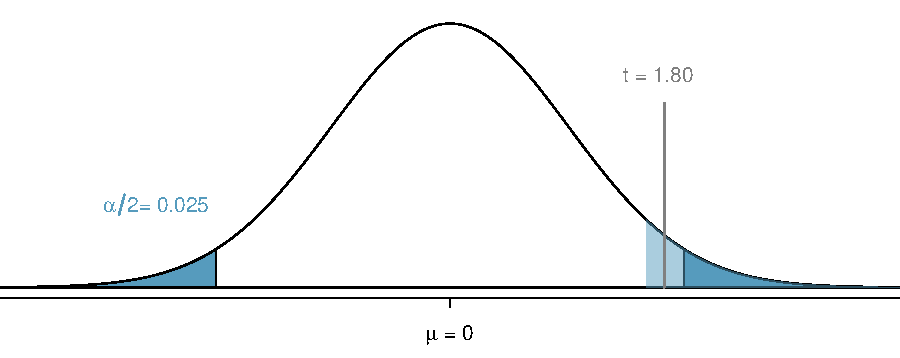
\includegraphics[width=0.9\textwidth]
	{ch_05a_inference_foundations_oi_biostat/figures/twoSidedTestConservative/twoSidedTestConservative}
	\caption{Under a one-sided test at significance level $\alpha$ = 0.05, a $t$-statistic of 1.80 is within the rejection region (shaded light blue). However, it would not be within the rejection region under a two-sided test with $\alpha$ = 0.05 (darker blue).}
	\label{twoSidedTestConservative}
\end{figure}

Two-sided tests are more "conservative" than one-sided tests; it is more difficult to reject the null hypothesis with a two-sided test. The $p$-value for a one-sided test is exactly half the $p$-value for a two-sided test conducted at the same significance level; as a result, it is easier for the $p$-value from a one-sided test to be smaller than $\alpha$. Additionally, since the rejection region for a two-sided test is divided between two tails, a test statistic needs to be more extreme in order to fall within a rejection region. While the $t$-statistic of 1.80 is not within the two-sided rejection region, it is within the one-sided rejection region.\footnote{The two-sided rejection regions are bounded by -1.96 and 1.96, while the one-sided rejection region begins at 1.65.}

%\textD{\newpage}

For a fixed sample size, a one-tailed test will have a smaller probability of Type II error in comparison to a two-tailed test conducted at the same $\alpha$ level. In other words, with a one-sided test, it is easier to reject the null hypothesis if the alternative is actually true. 

The choice of test should be driven by context, although it is not always clear which test is appropriate. Since it is easier to reject $H_0$ with the one-tailed test, it might be tempting to always use a one-tailed test when a significant result in a particular direction would be interesting or desirable. 

However, it is important to consider the potential consequences of missing a significant difference in the untested direction. Generally, a two-sided test is the safest option, since it does not incorporate any existing biases about the direction of the results and can detect a difference at either the upper or lower tail. In the 1980s, researchers were interested in assessing a new set of drugs expected to be more effective at reducing heart arrhythmias than previously available therapies. They designed a one-sided clinical trial, convinced that the newer therapy would reduce mortality. The trial was quickly terminated due to an unanticipated effect of the drug; an independent review board found that the newer therapy was almost 4 times as likely to kill patients as a placebo! In a clinical research setting, it can be dangerous and even unethical to conduct a one-sided test under the belief that there is no possibility of patient harm from the drug intervention being tested.

%cite two_tailed_clinical

One-sided tests are appropriate if the consequences of missing an effect in the untested direction are negligible, or if a large observed difference in the untested direction and a conclusion of "no difference" lead to the same decision. For example, suppose that a company has developed a drug to reduce blood pressure that is cheaper to produce than current options available on the market. If the drug is shown to be equally effective or more effective than an existing drug, the company will continue investing in it. Thus, they are only interested in testing the alternative hypothesis that the new drug is less effective than the existing drug, in which case, they will stop the project. It is acceptable to conduct a one-sided test in this situation since missing an effect in the other direction causes no harm. 

The decision as to whether to use a one-sided or two-sided test must be made before data analysis begins, in order to avoid biasing conclusions based on the results of a hypothesis test. In particular, changing to a one-sided test after discovering that the results are "almost" significant for the two-sided test is unacceptable. Manipulating analyses in order to achieve low $p$-values leads to invalid results that are often not replicable. Unfortunately, this kind of "significance-chasing" has become widespread in published science, leading to concern that most current published research findings are false.

%cite statistical_errors

%cite published_research_false


%\textD{\newpage}


\subsection{The informal use of $\pmb{\MakeLowercase{p}}$-values}
\label{informalUseOfp-values}

Formal hypothesis tests are designed for settings where a decision or a claim about a hypothesis follows a test, such as in scientific publications where an investigator wishes to claim that an intervention changes an outcome.  However, progress in science is usually based on a collection of studies or experiments, and it is often the case that the results of one study are used as a guide for the next study or experiment. 

Sir Ronald Fisher was the first to propose using $p$-values as one of the statistical tools for evaluating an experiment.  In his view, an outcome from an experiment that would only happen 1 in 20 times ($p$ = 0.05) was worth investigating further. The use of $p$-values for formal decision making came later.  While valuable, formal hypothesis testing can often be overused; not all significant results should lead to a definitive claim, but instead prompt further analysis.

The formal use of p-values is emphasized here because of its prominence in the scientific literature, and because the steps outlined are fundamental to the scientific method for empirical research: specify hypotheses, state in advance how strong the evidence should be to constitute sufficient evidence against the null, specify the method of analysis and compute the test statistic, draw a conclusion. These steps are designed to avoid the pitfall of choosing a hypothesis or method of analysis that is biased by the data and hence reaches a conclusion that may not be reproducible.


%_____________
\section{Notes}
\label{ch5Summary}

Confidence intervals and hypothesis testing are two of the central concepts in inference for a population based on a sample. The confidence interval shows a range of population parameter values consistent with the observed sample, and is often used to design additional studies. Hypothesis testing is a useful tool for evaluating the strength of the evidence against a working hypothesis according to a pre-specified standard for accepting or rejecting hypotheses.

The calculation of $p$-values and confidence intervals is relatively straightforward; given the necessary summary statistics, $\alpha$, and confidence coefficients, finding any $p$-value or confidence interval simply involves a set of formulaic steps. However, the more difficult parts of any inference problem are the steps that do not involve any calculations. Specifying appropriate null and alternative hypotheses for a test relies on an understanding of the problem context and the scientific setting of the investigation. Similarly, a choice about a confidence coefficient for an interval relies on judgment as to balancing precision against the chance of possible error. It is also not necessarily obvious when a significance level other than $\alpha = 0.05$ should be applied. These choices represent the largest distinction between a true statistics problem as compared to a purely mathematical exercise. 

Furthermore, in order to rely on the conclusions drawn from making inferences, it is necessary to consider factors such as study design, measurement quality, and the validity of any assumptions made. For example, is it valid to use the normal approximation to calculate $p$-values? In small to moderate sample sizes ($30 \leq n \leq 50$), it may not be clear that the normal model is accurate. It is even necessary to be cautious about the use and interpretation of the $p$-value. For example, an article published in \textit{Nature} about the mis-use of $p$-values references a published study that showed people who meet their spouses online are more likely to have marital satisfaction, with $p$-value less than 0.001. However, statistical significance does not measure the importance or practical relevance of a result; in this case, the change in happiness moved from 5.48 to 5.64 on a 7-point scale. A $p$-value reported without context or other evidence is uninformative and potentially deceptive.

%cite statistical_errors and asa_p_values

These nuanced issues cannot be adequately covered in any introduction to statistics. It is unrealistic to encourage students to use their own judgment with aspects of inference that even experienced investigators find challenging. At the same time, it would also be misleading to suggest that the choices are always clear-cut in practice. It seems best to offer some practical guidance for getting started:

\begin{itemize}
	\item The default choice of $\alpha$ is 0.05; similarly, the default confidence coefficient for a confidence interval is 95\%. 
	
	\item Unless it is clear from the context of a problem that change in only one direction from the null hypothesis is of interest, the alternative hypothesis should be two-sided.
	
	\item The use of a standard normal distribution to calculate $p$-values is reasonable for sample sizes of 30 or more if the distribution of data are not strongly skewed and there are no large outliers. If there is skew or a few large outliers, sample sizes of 50 or more are usually sufficient.
	
	\item Pay attention to the context of a problem, particularly when formulating hypotheses and drawing conclusions.
\end{itemize}

The next chapters will discuss methods of inference in specific settings, such as comparing two groups. These settings expand on the concepts discussed in this chapter and offer additional opportunities to practice calculating tests and intervals, reading problems for context, and checking underlying assumptions behind methods of inference.

%The labs for the chapter reinforce conceptual understanding of confidence intervals and hypothesis tests, and their link to sampling variability using the data from the YRBSS and NHANES. Both datasets are large enough to be viewed in an instructional setting as populations from which repeated samples can be drawn.  They are useful platforms for illustrating the conceptual role of hypothetical repeated sampling in the properties of tests and intervals, a topic which many students find difficult. Students may find the last lab for this chapter (Lab 4) particularly helpful for understanding conceptual details of inference, such as the distinction between the significance level $\alpha$ and the $p$-value, and the definition of $\alpha$ as the Type I error rate.

